\documentclass[a4paper]{article}

\usepackage[utf8]{inputenc}
\usepackage[T1]{fontenc}
\usepackage{textcomp}
\usepackage[english]{babel}
\usepackage{amsmath, amssymb}
\usepackage{listings}
\usepackage{minted}


% figure support
\usepackage{import}
\usepackage{xifthen}
\pdfminorversion=7
\usepackage{pdfpages}
\usepackage{transparent}
\newcommand{\incfig}[1]{%
	\def\svgwidth{\columnwidth}
	\import{./figures/}{#1.pdf_tex}
}

\pdfsuppresswarningpagegroup=1

\begin{document}
%%%%%%%%%%%%%% TODO: change all listings to mints
These notes pick up from chapter three. Notes on the content just before
this are in a physical notebook. 

\section{Distributed Memory Programming with MPI}
Start with a hello world program, taking inspiration from the classic
text by Kernighan and Ritchie.
\begin{minted}[frame=lines, linenos, fontsize=\large]
{c}
#include <stdio.h>
#include <string.h>
#include<mpi.h>

const int MAX_STRING = 100;

int main(void) {
	char greeting[MAX_STRING];  
	int comm_sz;  // number of processes
	int my_rank;

	MPI_Init(NULL, NULL);
	MPI_Comm_size(MPI_COMM_WORLD, &comm_sz);
	MPI_Comm_rank(MPI_COMM_WORLD, &my_rank);

	if (my_rank != 0) {
		sprintf(greeting, "Greetings from process %d of %d!",\
			 my_rank, comm_sz);
		MPI_Send(
			greeting, /* message buffer*/
			strlen(greeting)+1,  /* message size */
			MPI_CHAR,  /* message type */
			0, 0,  /* destination (rank) and tag
			MPI_COMM_WORLD  /* communicator */);
	} else {
		printf("Greetings from process %d of %d!", my_rank,\
			comm_sz);
		for (int q = 1; q < comm_sz; q++) {
			MPI_Recv(greeting, MAX_STRING, MPI_CHAR,\
				q,\  /* source */
				0,\  /* tag */ 
				MPI_COMM_WORLD,\  /* communicator */
				MPI_STATUS_IGNORE /* status_p */);
			printf("%s\n", greeting);
		}
	}
}
\end{minted}

I have already installed all the required libraries and binaries. For
the remainder of this chapter, \texttt{mpicc} will be used for compiling
assembling and linking everything. It's our GCC for programs that use
\texttt{\#include<mpi.h>}.

Compile using\\
\texttt{\$ mpicc -g -Wall -o mpi\_hello mpi\_hello.c}

I checked \texttt{man mpicc} and it says nothing about optimization
flags. mpicc is a wrapper for some C compilation pipeline, and most
likely handles that for us. Note that we didn't have to use \texttt{-lmpi}
or something like that to link \texttt{mpi.h}.

So, if the generated executable object file is executed simply like
you would normally as in \texttt{./mpi\_hello}, it'll just treat
it as a single process task. Some systems provide alternative 
program startup methods e.g. \texttt{mpiexec}\\
\texttt{\$ mpiexec -n <number of processes> ./mpi\_hello}

So, if I try running with six processes, I get this on my terminal
\lstinputlisting{ch03/hello_out.txt}

BTW, my machine has 1 socket, 6 physical cores and two threads per core.
So, if I load up bashtop, it shows me a total of twelve cores available
and in use. But, when I try to \texttt{mpi\_hello} for with more than
six processes, I get the following error
\lstinputlisting{ch03/hello_out_err.txt}

The second to the last paragraph seems interesting. Let's try it out
for 12 processes
\lstinputlisting{ch03/hello_out_12.txt}

Fuck yeah!

So, back to what we were doing. While we are using \texttt{mpiexec}
to execute a specific number of instances of the program, it can also
be used to tell the system which core should run each instance of the
program.


Now of course we should take a look at what exactly the code is doing.
Note that all the identifiers in \texttt{mpi.h} start with the prefix
\texttt{MPI\_} and I really hope that there are no exceptions to this.
Macros and constants are all upper case, and other constructs are a
mix of snake\_case and CamelCase.

\subsection{\texttt{MPI\_Init} and \texttt{MPI\_Finalize}}
No other MPI function should be called before the initializing
function, and no MPI function should be called after the finalizing
function.

These functions don't necessarily have to be in \texttt{main}

The initializer does the necessary setup like storage allocation for message buffers, 
rank allocation etc.

The syntax is\\
\begin{minted}[frame=lines, linenos, fontsize=\large]
{c}
int MPI_Init(
	int* argc_p,  // in/out
	char *** argv_p);  //in/out
\end{minted}

These are essentially pointers to \texttt{argc} and \texttt{argv}.
We can pass \texttt{NULL} when our program doesn't use these. The
\texttt{int} retval is error codes, i.e. in the same vein as main
returning \texttt{int}. We won't really need those error codes.
Hopefully.

\texttt{MPI\_Finalize} is to \texttt{MPI\_Initialize} what \texttt{free} 
is to \texttt{malloc}.

\subsection{Communicators, \texttt{MPI\_Comm\_size} and \texttt{MPI\_Comm\_rank}}
A \textbf{communicator} is a collection of processes that can send
messages to each other. One of the purposes of \texttt{MPI\_Init} is
to define a communicator (\texttt{MPI\_COMM\_WORLD}) that consists of all the processes started
when the program begins execution. Their signature is 

\begin{minted}[frame=lines, linenos, fontsize=\large]
{c}
int MPI_Comm_size(
	MPI_Comm comm,  /* in */
	int *comm_sz_p  /* out */);
int MPI_Comm_rank(
	MPI_Comm comm,  /* in */
	int *my_rank_p  /* out */);
)
\end{minted}

Again, \texttt{int} retval because error codes, and the desired values,
the number of processes and the calling process' rank, are stored in
the variable pointed to by the second argument.

\subsection{Communication}
The first branch of the \texttt{if-else} block generates a message
and sends it to process 0. The next branch is executed only for
process 0 and receives and prints the messages received from processes
\texttt{1..=p}.
\subsubsection{\texttt{MPI\_Send}}
It can be seen that the signature is somewhat complex. The first three
arguments are the message buffer, size and type in that order. The
remaining arguments are desitnation, tag and communicator, in that
order. \texttt{strlen+1} is used to make space for the terminating
null character.

Now, why do we need a special datatypes for the MPI functions? Because
standard CeeLanguage datatypes can't be passed to functions. So, I guess
that they used structs or enums to implement these types. The type
of these datatypes is MPI\_Datatype, which perhaps would have been
called MPI\_Datatype\_t if it were up to some other people to name it.
In addition to the standard CeeLanguage datatypes, MPI also has an
MPI\_Packed.

Tag is just an argument used for distinguishing different types of
messages from the same process. Kind of like identifiers for buffers
in FORTRAN.

The last argument is the communicator. So, a message sent by a
process via one communicator can't be received by a process using
another communicator.

\subsubsection{\texttt{MPI\_Recv}}
The first six arguments correspond to the six arguments of the sender.
Instead of destination, there's a source. There's another parameter
called \texttt{status\_p}, which will be discussed later.

\subsubsection{Message Matching}
The message sent by rank $q$ will be received by a process ranked $p$
using the appropriate function calls only if
\begin{itemize}
	\item \texttt{recv\_comm = send\_comm}
	\item \texttt{recv\_tag = send\_tag}
	\item \texttt{dest = r}
	\item \texttt{src = q}
\end{itemize}

Yup, makes sense to me. The first three parameters also play an important
role, because conflicts over there  would basically mean conflicting
datatypes, buffer spaces etc.. If they don't match, then there is a risk
of segfaulting or stack smashing. For now, one just has to make sure
that the received and sent types are the same and the receiving buffer
is larger than (or same size as) the sender's buffer.

The receiver function can also accept some wildcard arguments in the
cases when it doesn't matter in which order or from what tags messages
are received. So, the \texttt{src} could be \texttt{MPI\_ANY\_SOURCE},
with the \texttt{status\_p} argument set to \texttt{MPI\_STATUS\_IGNORE}. Similarly there's also a \texttt{MPI\_ANY\_STATUS} etc.

%%%%%%%%%%%%%% TODO: add notes on status_p and things that can go wrong
\subsubsection*{The  \texttt{status\_p} argument }
The only contraints for receiving messages are the four specified
above. Messages can still be received if the first three arguments 
differ between corresponding send and receive. 

The last argument \texttt{MPI\_Recv} has type \texttt{MPI\_Status*},
where \texttt{MPI\_Status} is a struct with at least the three members
\texttt{MPI\_SOURCE}, \texttt{MPI\_TAG}, and \texttt{MPI\_ERROR}.
So, if a status argument is passed to the receiver function, then
we can determine the sender and tag using
\begin{center}
	\texttt{status.MPI\_SOURCE}\\
	\texttt{status.MPI\_TAG}
\end{center}

This leaves the data size, which can be retrieved with a call to
\texttt{MPI\_Get\_count}. The call goes like
\begin{center}
\texttt{MPI\_Get\_count(\&status, recv\_type, \&count)},
\end{center}
where \texttt{recv\_type} is the type of the receive buffer in the 
\texttt{MPI\_Recv} call. \texttt{count} then identifies the message
length.

So, basically they're just calculating the buffer length in terms
of the number of data entries of the given datatype. Nothing fancy
going on here.

\subsection*{Example - Trapezoidal Rule}
Remember the Trapezoidal rule? A quick and dirty way of numerically
integrating nice functions. We are going to write the sequential code
before moving on to the MPI implementation.

\subsubsection*{The trapezoidal rule}
We want to numerically evaluate
\begin{equation}
	\int_a^b f(x) \mathrm{d} x
\end{equation}
by partitioning the interval $\left[ a, b \right] $ uniformly into
$n$ subintervals. Let $\left\{ x_i \right\} \forall i \in n$ do
the partitioning. (\textit{Note: if $n \in  \mathbb{N}$,  then $i \in n$ means $i \in  \left\{ 0, 1, 2, \ldots n \right\} $, a notation
that I have seen in some mathematics literature}). This also
partitions the area under the curve and you know what the trapezoids
in the trapezoid rule are.

Area of one trapezoid is
\begin{equation}
	\frac{h}{2}\left[ f(x_i)+f(x_{i+1}) \right] ]
\end{equation}
where $h = \frac{b-a}{n}$, so that
\begin{equation}
	\begin{split}
		x_0 &= a\\
		x_1 &= a + h\\
		x_2 &= a + 2h\\
		    &\vdots \\
		    x_n &= a + nh = b
	\end{split}
\end{equation}

So, the approximate area under the curve is given by 
\begin{equation}
	h \left[ \frac{f(x_0)}{2} + f(x_1) + f(x_2) + \ldots + f(x_{n-1}) + \frac{f(x_n)}{2} \right]
\end{equation}

So, a sequential code would look something like this
\begin{minted}[frame=lines, linenos, fontsize=\large]
{c}
/* Input: a, b, n */
h = (b-a)/n;
approx = (f(a) + f(b))/2.0;
for (i = 1; i < n; i++) {
	x_i = a + i*h;
	approx += f(x_i);
}
appox = h*approx;
		
\end{minted}

EZ.

\subsubsection*{Parellelizing the trapezoidal rule}
Recall the four basic steps
\begin{enumerate}
	\item Partition the solution into tasks
	\item Identify the communication channels between the tasks
	\item Aggregate the tasks into composite tasks
	\item Map the composite tasks to cores
\end{enumerate}

Say we have some \texttt{comm\_sz} cores at our disposal. If
\texttt{comm\_sz} evenly divides $n$, then great, else we will have
to stick to floor division.

Here is what the parallel pseudo code looks like
\begin{minted}[frame=lines, linenos, fontsize=\large]
{c}
h = (b - a)/n;
local_n = n/comm_sz;
local_a = a + my_rank*local_n*h;
local_b = local_a + local_n*h;
local_integral = Trap(local_a, local_b, local_n, h);
if (my_rank != 0) {
	send(local_intergal, process0);
} 
else {
	for (proc = 1; proc < comm_sz; proc++) {
		receive(local_intragral, proc);
		total_integral += local_integral;
	}
}

if (my_rank == 0)
	print(result);
\end{minted}

Which translates to the following \texttt{main} in the MPI program
with hardcoded values instead of inputs
\begin{minted}[frame=lines, linenos, fontsize=\large]
{c}
int main() {
	int my_rank, comm_sz = 1024, local_n;
	double a = 0.0, b = 3.0, h, local_a, local_b;
	double local_int, total_int;
	int source;

	MPI_Init(NULL, NULL);
	MPI_Comm_rank(MPI_COMM_WORLD, &my_rank);
	MPI_Comm_size(MPI_COMM_WORLD, &comm_sz);

	h = (b-a)/n;
	local_n = n/comm_sz;
	local_a = h;
	local_b = local_a + local_n*h;
	local_int = Trap(local_a, local_b, local_n, h);

	if (my_rank != 0 ) {
		MPI_Send(&local_int, 1, MPI_DOUBLE, 0, 0, MPI_COMM_WORLD);
	} else {
		total_int = local_int;
		for (source = 1; source < comm_sz; source++) {
			MPI_Recv(&local_int, 1, MPI_DOUBLE, source, 0, PMI_COMM_WORLD, MPI_STATUS_IGNORE);
		total_int += local_int;
		}
	}

	if (my_rank == 0 ) {
		printf("With n = %d trapezoids, our estimate\n", n);
		printf("of the integral from %f to %f = %.15e\n", a, b, total_int);
	}
	return 0;
}

double Trap {...} {...};
\end{minted}

\subsubsection*{Semantics of \texttt{MPI\_Send} and \texttt{MPI\_Recv}}
Once a sending process assembles a message, with the message and the
metadata (e.g. sending process rank, destination rank, datatype and
all that), it can either \textbf{buffer} the message, or \textbf{block}. 
\begin{itemize}
	\item \textbf{buffer}: MPI places the assembled message into
		some internal storage and the sending process
		can move on to the next instruction, i.e. the call to
		\texttt{MPI\_Send} returns.
	\item \textbf{block}: process waits until it can begin transmitting
		the message, i.e. till a matching receiver is found. 
\end{itemize}

When a call to \texttt{MPI\_Send} returns, it cannot be said whether
the message has been transmitted or not, it simply means that the
send buffer is now available for use again. There are separate functions for knowing whether the message has been
transmitted or not, or if we want to explicitly buffer et cetera.

Quite sensibly, \texttt{MPI\_Recv} always blocks. MPI messages are
non-overtaking, i.e. if $q \text{ and } r$ are two processes and
$q$ sends two messages to $r$ in succession, then $r$ must receive them
in the same order in which they were sent, but if messages from different
processes can be received by a single receiving process in any order.

The system can \textbf{hang} if there is no matching receive to a
\textbf{blocking} send. This could happen if there are errors in
values of tags, process ranks et cetera.
Alternatively, if a \textbf{buffering} send does  not have a matching
receive, then the message is lost forever. RIP. A mismatched receive
could also end up receiving from the wrong process, which might
cause all sorts of havoc.

\subsection*{Dealing with I/O}
The MPI standard does not define which processes have access to
I/O devices, so it is a good practice to pick a good convention and
follow it. E.g. process 0 can write to \texttt{stdout} and we try to
use nothing else to print to \texttt{stdout}.

Pretty much all the processes in \texttt{MPI\_COMM\_WORLD} have
full access to \texttt{stdout} and \texttt{stderr}.
But, you cannot expect an MPI implementation to also do the access
scheduling to these devices for you; the OS will handle that and
the output for runs with identical inputs will be `nondeterministic'.

As an example, consider the simple program
\begin{minted}[frame=lines, linenos, fontsize=\large]
{c}
#include <stdio.h>
#include <mpi.h>

int main(void) {
	int my_rank, comm_sz;

	MPI_Init(NULL, NULL);
	MPI_Comm_size(MPI_COMM_WORLD, &comm_sz);
	MPI_Comm_rank(MPI_COMM_WORLD, &my_rank);

	printf("Proc %d of %d > Does anyone have a toothpick?\n",
		my_rank, comm_sz);
	MPI_Finalize();

	return 0;
}
\end{minted}

Just another hello world program, right? Well, see the screenshot in Figure \ref{fig:indet}.

\begin{figure}[h]
	\centering
	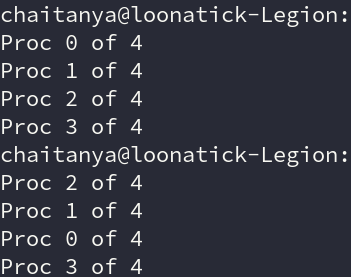
\includegraphics[width=0.4\textwidth]{figures/indeter.png}
	\caption{Allowing all processes to use \texttt{stdout}}
	\label{fig:indet}
\end{figure}

Most MPI implementations allow only process 0 to access \texttt{stdin}. So, values from \texttt{stdin} will have to be shared with other
prcesses through message passing from process 0.

So, if it is statically known that all processes must receive the input,
one could write a function that does the input receiving from
\texttt{stdin}, the \texttt{MPI\_Send} to other processes and
\texttt{MPI\_Recv} from process 0. Writing the funcion down for
practice
\begin{minted}[frame=lines, linenos, fontsize=\large]
{c}
void Get_input(
	int my_rank, int comm_sz,
	double *a_p, double *b_p,
	int *n_p) {
		int dest;

		if (my_rank == 0) {
		printf("Enter a, b, and n\n");
		scanf("%lf %lf %d", a_p, b_p, n_p);
		for (dest = 1; dest < comm_sz; dest++) {
			MPI_Send(a_p, 1, MPI_DOUBLE,
				0, 0, MPI_COMM_WORLD);
			MPI_Send(b_p, 1, MPI_DOUBLE,
				0, 0, MPI_COMM_WORLD);
			MPI_Send(n_p, 1, MPI_INT,
				0, 0, MPI_COMM_WORLD);
			}
		} else {
			MPI_Recv(a_p, 1, MPI_DOUBLE,
				0, 0, MPI_COMM_WORLD);
			MPI_Recv(b_p, 1, MPI_DOUBLE,
				0, 0, MPI_COMM_WORLD);
			MPI_Recv(n_p, 1, MPI_INT,
				0, 0, MPI_COMM_WORLD);
		}
	}
\end{minted}

Yeah, this is a funcion with a lot of side effects, but I do not have
enought development experience to know how good or bad this practice
is and whether there is a recommended alternative.

\subsection*{Collective communicaion}
The parallelization proposed is for the trapezoidal rule is not the
most efficient one that we can think of; having process 0 do all the
sequential work and the rest quit is not optimum. Remember Amdahl's
law? For a sequential program of which a proportion $p$ can be parallelized,
the maximum possible speedup (i.e. assuming all the good stuff like
load balancing, low latency, low communication overheads et cetera) is
\begin{equation}
	S(N) = \frac{1}{\frac{p}{N} + 1-p}
\end{equation}
where $N$ is the number of nodes/cores at our disposal. So, for
$n > N$ intervals, the length of each parallel branch is $n/N$, while
the final sequential branch has length $N$, giving a total length
of $n/N + N$. (Here the loosely used term `length' is a measure of running time)

The same program when executed sequentialy has length $n$.
The speedup is then loosely speaking
\begin{equation} \label{firstgear}
	S(N) = \frac{n}{\frac{n}{N} + N}
\end{equation}

It is possible
to improve the program by further parallelizing the sequential
part. Better yet, we could come up with a different algorithm altogether,
because na\"ive parallelization can make the program slower instead.

\subsubsection*{Tree structured communication}
Remember fast adders from EE 224? This kind of reminds me of those. I'm
sure that this will be unfounded if I sit down to revise Professor
Viru's notes L\"OL.
Say, we have 8 processes, 0 through 7. Each of them has computed a
local sum of its own. 

The even numbered processes then receive
the local sum of the next odd numbered process and add it to their
local sum to create a new local sum. The number of partial sums is
halved. Repeat for the remaining partial sums to get the complete sum.

Figure \ref{fig:improve} shows this
\begin{figure}[h]
	\centering
	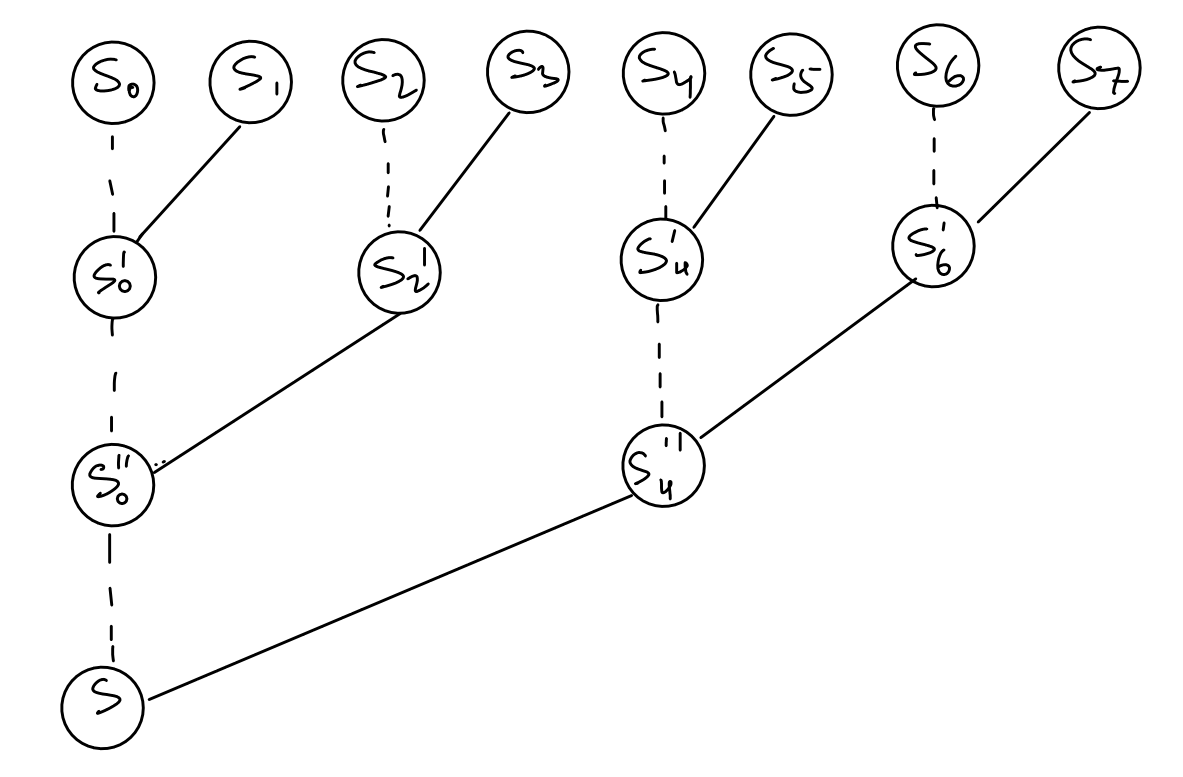
\includegraphics[width=0.8\textwidth]{figures/improve.png}
	\caption{A better parallel algorithm for getting completet sum
	from partial sums}
	\label{fig:improve}
\end{figure}

So, instead of a single set of parallel branches, we have multiple parallel branches.
The length of the first set is still $n / N$, while the sequential
part goes down from $n$ to $\log n$. This is a significant speedup
of the sequential section for larger values of $n$.

Implementing such tree structured stuff is not as easy as the na\"ive
method of course. Multiple topologies are possible. E.g. Figure \ref{fig:figures-topo-png}
\begin{figure}[h]
	\centering
	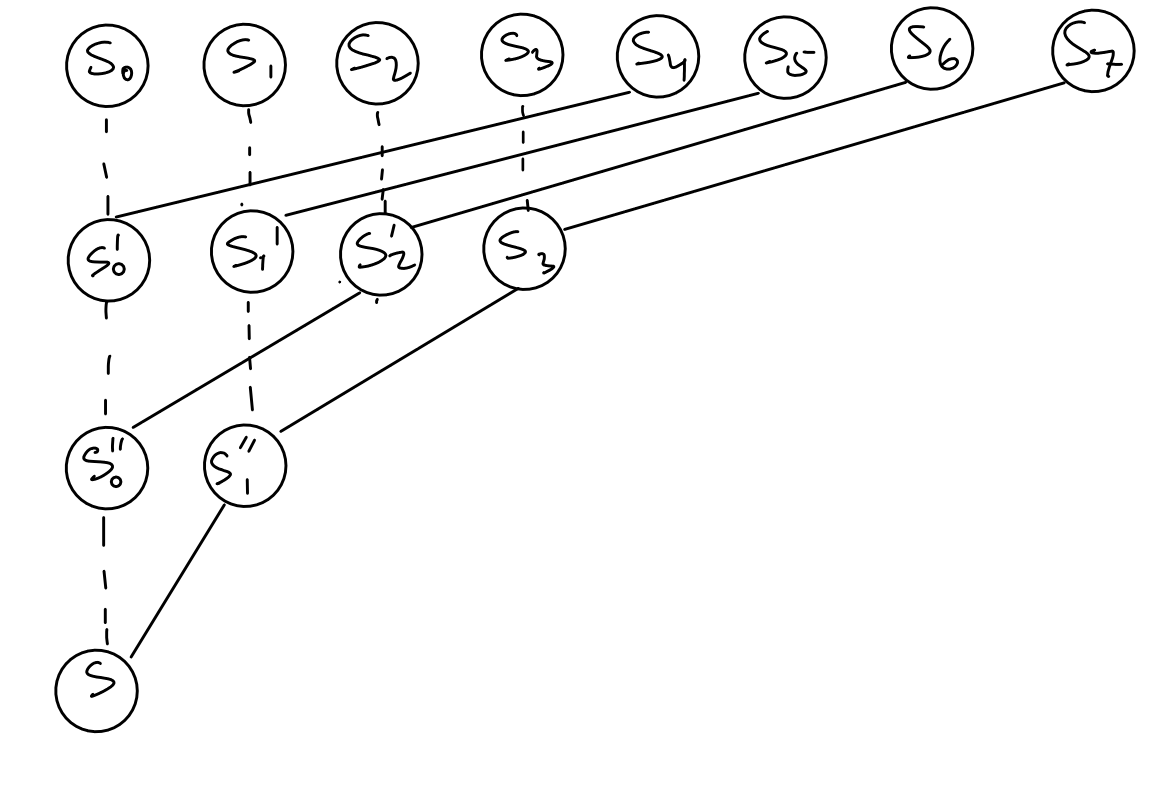
\includegraphics[width=0.8\textwidth]{figures/topo.png}
	\caption{Alternative tree topology that gives the same runtime}
	\label{fig:figures-topo-png}
\end{figure}

Smells like lots of boilerplate incoming. Unless\ldots

\subsubsection*{\texttt{MPI\_Reduce}}
MPI standard includes implementations of global sums. GG. The application
programmer hopes that the developer of the MPI implementation knows
what they are doing.

Such global functions that involve the communication of more than two
processes (i.e. unlike \texttt{MPI\_Send}, \texttt{MPI\_Recv} pairings)
are called \textbf{collective communications} (as opposed to \textbf{point-to-point} communication).

The function \texttt{MPI\_Reduce} takes in addition to the usual
parameters, an operator parameter. The previous code would be equivalent
to the function call
\begin{minted}[frame=lines, linenos, fontsize=\large]
{c}
double local_x[N], sum[N];
/*
...
*/
MPI_Reduce(local_x, sum, N, MPI_DOUBLE, MPI_SUM, /* operator */
		0, MPI_COMM_WORLD);	
\end{minted}

Some important points about collective and one-to-one communcations
\begin{itemize}
	\item All the processes in the communicator must call the same
		collective function; a program cannot have a call to
		\texttt{MPI\_Reduce} in one process and an equivalent
		call to \texttt{MPI\_Recv} on another
	\item placeholder
\end{itemize}
For more information check out \texttt{man MPI\_Reduce}.
There are some other topologies as well, e.g. butterfly et
cetera. Not documenting everything here. Check out the man pages
\texttt{SEE ALSO} sections to get to know them.


\subsection*{Derived Datatypes in MPI}
Sending a series of builtin datatypes using a series of Send-Receives
is a lot more expensive than sending all the data in a single 
send-receive. This can be done by defining your own datatype that
is optimized for use in MPI. It is not as straightforward as just
packaging everything in a struct.

We use \texttt{MPI\_Type\_create\_struct} to create such derived
datatypes.

\begin{minted}[frame=lines, linenos, fontsize=\large]
{c}
int MPI_Type_create_struct(
	int count  /* in */,
	int array_of_block_lengths[]  /* in */,
	MPI_Aint array_of_displacements[]  /* in */,
	MPI_Datatype array_of_types[]  /* in */,
	MPI_Datatype* new_type_p  /* out */)
\end{minted}

\begin{itemize}
	\item \texttt{count}: Number of elements in datatype
	\item \texttt{array\_of\_block\_lengths}: in case individual elements are themselves arrays, pass
		\texttt{{1, 1, 1, \ldots}} if all scalars.
	\item \texttt{array\_of\_displacements}: displacement of each type from beginning of message
	\item \texttt{array\_of\_types}: types of individual elements
\end{itemize}

The second argument essentially means that arrays in  the datatype
must have fixed lengths. To find what to use for the third argument,
\texttt{MPI} provides  \texttt{MPI\_Get\_address}.

\begin{minted}[frame=lines, linenos, fontsize=\large]
{c}
int MPI_Get_address(
	void* location_p  /* in */,
	MPI_Aint* address_p  /* out */);
\end{minted}

So, if we want a derived datatype made of some three datatypes, the
$i^{\text{th}}$ element of the displacements array is the difference 
between the output of
\texttt{MPI\_Get\_address} for the $i^{\text{th}}$ data and
the output for the first data.

Before the new datatype is ready for use, you first have to \textbf{commit}
it using \texttt{MPI\_Type\_commit}. This allows for optimization of
internal representation of the derived datatype for use in message passing.
It can then be sent and received like any other MPI datatype.

\subsection*{Parallel Sorting Algorithm}
First things first, what is the input? What is the output? The answer
depends on where the keys are stored. We can start or finish with
the keys distributed in different processes, or we can collect them
in the same process.

If we have a total of $n$ keys and $p = $\texttt{comm\_sz} processes,
our algo will start and finish with $n/p$ keys assigned to each process.
When the algorithm terminates, 
\begin{itemize}
	\item  the keys assigned to each process
		will be sorted
	\item if $0\le q < r < p$, then each key assigned to process
		$q$ should be less than equal to each key assigned
		to process $r$
\end{itemize}

Consider bubble sort. It is as sequential as it gets and it doesn't
make sense parallelizing it. But, there is a variant of the bubble
sort called the \emph{odd-even transposition sort}, the key idea
being decoupling of the compare-swap.
\begin{itemize}
	\item Even phase: compare-swap at indices, $2j$, $2j+1$ 
	\item Odd phase: compare-swap at indices $2j+1$, $2j+2$
\end{itemize}
It can be shown that the array will be sorted in at most $n$ phases.
An even phase followed by an odd phase constitutes one pass. So,
So, each pass has a sequence of two parallel stages in series.
For a parallelized version with $p$ processes, the array will be 
sorted in $p$ phases (assuming $p$  divides $n$).

In general, during even phases, odd-reanked partners exchange with
 \texttt{my\_rank-1} and even-ranked partners exchange with
 \texttt{my\_rank+1}. There are going to be edge cases for 
 ranks 0 and  \texttt{comm\_sz-1}.

\subsubsection*{Safety}
The MPI standard allows \texttt{MPI\_Send }to behave in two ways - blocking
and buffering. Many systems set a threshold at which the system
switches from buffering to blocking; small messages are buffered
while larger ones are blocking. So, we can easily have hangs
and deadlocks if we are not careful. In conclusion, \texttt{MPI\_Send} is \emph{unsafe} 
because it relies on MPI provided buffering  Thankfully, MPI
provides safer alternatives in the form of synchronous send - \texttt{MPI\_Ssend}.

%%%% TODO: the whole commentary on MPI_Ssend, MPI_Sendrecv etc, and merge

\begin{minted}[frame=lines, linenos, fontsize=\large]
{c}
void Merge_low(
		int my_keys[],  /* in/out */
		int recv_keys[],  /* in */
		int temp_keys[],  /* scratch */
		int local_n  /* = n/p, in */) {
	int m_i, r_i, t_i;
	m_i = r_i = t_i = 0;
	while (t_i < local_n) {
		if (my_keys[m_i] <= recv_keys[r_i]) {
			temp_keys[t_i] = my_keys[m_i];
			t_i++; m_i++;
		} else {
			temp_keys[t_i] = recv_keys[r_i];
			t_i++; r_i++;
		}
	}

	for (m_i = 0; m_i < local_n; m_i++) {
		my_keys[m_i] = temp_keys[m_i];
	}
}
\end{minted}
\end{document}

\subsection*{Attempts at Exercises}

